\documentclass[12pt,a4paper]{article}
\usepackage[utf8]{inputenc}
\usepackage{amsmath}
\usepackage{amsfonts}
\usepackage{amssymb}
\usepackage{graphicx}
\usepackage{booktabs}
\usepackage{natbib}
\usepackage{dcolumn}
\usepackage{setspace}
\usepackage{array}
\usepackage{pdflscape} %allows for rotating pages with wide tables
\newcolumntype{P}[1]{>{\raggedright\arraybackslash}p{#1}}
%\usepackage{tabulary}
\usepackage[T1]{fontenc}
\usepackage{lmodern}
\usepackage{multirow}
\usepackage{multicol}
\usepackage{todonotes}

%\usepackage{mathptmx} %times font
\usepackage{tgpagella} %times font
\usepackage[protrusion=true,expansion=true]{microtype}
\usepackage[top=1in, bottom=1in, left=1in, right=1in]{geometry}
\usepackage[hidelinks]{hyperref}
\usepackage{color,soul} %highlighting
\usepackage{caption}
\captionsetup[figure]{labelfont=bf}
\captionsetup[table]{labelfont=bf}

%\usepackage{endnotes}
%\usepackage[heads,nolists,tablesfirst]{endfloat} %places tables and figures at the end
%

%%making use of footnotesize in all tables
\usepackage{floatrow}
\DeclareFloatFont{tiny}{\footnotesize}% "scriptsize" is defined by floatrow, "tiny" not
\floatsetup[table]{font=footnotesize}

%putting caption on top
\usepackage{float}
\floatstyle{plaintop}
\restylefloat{table}

\usepackage{epstopdf}

\title{\textbf{Housing Bubbles and \\Support for Incumbents}}


\author{Martin Vinæs Larsen\thanks{Corresponding author. \href{mailto:mvl@ifs.ku.dk}{\texttt{mvl@ifs.ku.dk}}. } \qquad Frederik Hjorth \qquad Peter Thisted  Dinesen \\Department of Political Science \\ University of Copenhagen \and Kim Mannemar  Sønderskov  \\Department of Political Science \\ Aarhus University   }

%,  }  } 


\begin{document}

\maketitle

\begin{center}
	\textsc{Presented at the 2016 Annual Meeting  \\
	of the American Political Science Association \\
	September 1-3, Philadelphia, PA \\[1em]
	please only quote or cite with permission}
\end{center}

\begin{abstract} The state of the economy - one’s own or that of the nation - has long been considered among the most important predictors of support for incumbent politicians. While a simple idea at heart, the specifics of retrospective voting remain debated. In this paper, we focus on what we believe to be an understudied economic influence: local housing markets. We propose that housing markets shape voting by providing locally derivable information about incumbent politicians’ capacity to manage the economy, and test this proposition by examining the relationship between changes in the local housing market and support for the incumbent government in Denmark. Linking uniquely detailed and comprehensive data on housing sales at the local level to both precinct-level election returns and a two-wave panel survey, we find the hypothesized positive relationship between local housing prices and support for governing parties.
 
\end{abstract}






%\begin{keyword}
%\doublespacing
%%x \sep y
%\end{keyword}

%\end{frontmatter}

\newpage

%\onehalfspacing
\doublespacing

\section{Introduction}

The state of the economy - one’s own or that of the nation - has long been considered among the most important predictors of support for incumbent politicians. This is generally considered desirable because it provides a shorthand for evaluating the performance of incumbent politicians and punish and reward them accordingly \citep{ashworth2012electoral,healy2013retrospective}. While a simple idea at heart, the specifics of retrospective voting remain debated. In this paper, we focus on what we believe to be an understudied economic influence: local housing markets. 

Housing markets saw a global boom followed by a bust in the period around the great recession. This had severe economic implications for well-being of both individual households and the overall state of the economy. Pairing the economic importance of the housing market with the fact that national housing and monetary policy to a considerable extent influenced the severity of the market crash makes housing markets a particularly useful mean for voters to evaluate the incumbent government by. Furthermore, housing markets are not a monolithic national phenomenon, but vary substantially across geographical contexts, thereby providing voters with relevant local information by which to assess incumbents. 

In this paper, we assess the relationship between changes in the local housing market and support for the incumbent government in Denmark, using uniquely detailed and comprehensive data on housing sales at the local level. We do this using two complementary empirical approaches. First, we link detailed registry data on local housing prices to election results at the precinct level across four national elections, allowing us to study whether within-district differences in property values are related to support for parties in government. Second, to test the hypothesized causal mechanism that voters make inferences about government based on the state of their local housing market, we zoom in on individual voters' local contexts. Specifically, we link a two-period panel survey to precise measures of how individuals' neighborhoods --measured at very low levels of aggregation-- were affected by changes in house prices.

We find the hypothesized positive relationship between local housing prices and support for governing parties at both the precinct-level and in the individual-level data. Specifically, a 50 pct. year-on-year increase in local housing prices, equivalent to the sharpest price increases during the housing boom, is associated with a 3 to 5 percentage points increase in the support for governing parties. In subsequent analyses, we probe the suggested role of local housing markets further by testing a number of observable implication arising from this conjecture. We find no evidence that housing prices affect the respondents ideological orientation, and no evidence that the effect of housing prices on incumbent support depends on whether you own your own home. Instead, our analyses suggest that the effect of housing prices is more pronounced among individuals who are more likely to be attuned to the state of their local housing market -- in effect those have recently or who will soon be relocating. Taken together, these analyses seem to suggest that voters do not respond to changes in local housing prices because it changes their preferences for specific policy interventions or their own economic situation, but because of what the the local housing market tells them about incumbents capacity to manage the economy in a way that benefits their community.

 %A contribution to extant research which has focused on the extent to which voters draw such inference from how policy affects the national economy \citep[e.g.][]{fiorina1981retrospective,duch2008economic}, and to a lesser extent, their own personal economy \citep[e.g.][]{kinder1981sociotropic,markus1988impact}. 






\section{Relation to existing literature}

We are not the first to investigate, whether voters might draw inferences about policy outcomes from local economic conditions. A number of studies have examined the extent to which voters draw inferences about national economic conditions from local economic conditions \citep{books1999contextual,reeves2012ecologies,anderson2011local,ansolabehere2014mecro,bisgaard2016reconsidering}, and a number of studies have examined the extent to which voters draw inferences about whether to support incumbent politicians  \citep{hansford2015reevaluating,eisenberg2004economic,kim2003spatial,healy2014presidential}. The results from these studies are somewhat mixed, but on balance they find that voters do make inferences based on local economic conditions; asserting that the national economy declining or that incumbent politicians are doing a bad job when local economic conditions are declining. 

Our study distinguishes itself from these previous efforts by focusing specifically on the role of local housing markets, not just individual home ownership and the personal economic asset it constitutes, in shaping support for incumbents. Theoretically, we thus highlight how housing markets -- in addition to concerns over personal finances already established in the literature -- shape voting by providing locally derivable information about incumbent politicians’ capacity to manage the economy.

In doing so, our study ties into several neighboring literatures. First, a recently emerged strand of research in political economy highlighting the influence of home ownership -- in itself or as part of a portfolio of economic assets -- on redistribution and social policy preference as well as voting \citep{ansell2014political,nadeau2010patrimonial,stubager2013reaching}. Second, by conceptualizing housing bubbles as the result of government policy, our study also relates to the policy feedback literature \citep{campbell2012policy,mettler2004consequences,pierson1993effect}, which emphasizes how policies shape mass political behavior by providing incentives and conveying information to citizens.

At the methodological level, we contribute to the existing literature by exploiting uniquely detailed and comprehensive data on housing market transactions available in Danish public registries. Specifically, we can link highly detailed register data on local housing prices to both precinct-level panel data on national election outcomes as well as individual-level panel survey data. These data ameliorate three immanent methodological challenges confronting the broader class of studies scrutinizing local influences on political attitudes and behavior.

First, using extremely precise and highly local measures of house prices enables us to address the common problem of confounding of local context with local media market—a very different mechanism—typically arising in previous studies focusing on local economic conditions in highly aggregate geographical contexts (due to limited data availability) \citep[][]{bisgaard2016reconsidering}.  

Second, and related to the previous point,  measures of local economic conditions are often based on samples which, while large enough to estimate precise national economic conditions, typically suffer from insufficient precision when estimating conditions at lower geographical levels \citep[][]{healy2014presidential}. 

Third, the panel set-up of data enables us to rule out time-invariant structural differences between local contexts as explanations of any observed relationship between local house prices and support for incumbents by using only within-precinct/individual variation in local housing prices (by means of fixed effects). This is particularly important given the strong urban-rural gradient in local property values, which would very likely confound any observed cross-sectional relationship with support for the sitting government. 

While some previous studies do  some of these methodological challenges, our study is to the best of our knowledge the first to address all of these shortcomings at once. 



\section{Empirical setting: a policy-driven boom and bust}

The setting of our study is Denmark in the years surrounding the onset of the Great Recession. The precinct-level data (cf. Section \ref{precinctlevel}) covers the election years of 2005, 2007, 2011, and 2015, whereas the individual-level data (cf. Section \ref{individuallevel}) covers panel survey responses from 2004, 2008, and 2011. Studying the relationship between changes in housing prices and support for the incumbent government in Denmark in this period of time is useful due to large temporal variations in these prices. The boom and bust of the Danish real-estate market before and during the great recession was very dramatic, even by international standards. Figure \ref{dam} shows the trajectory of Denmark's housing bubble compared with other international cases.



\begin{figure}[htbp!]
	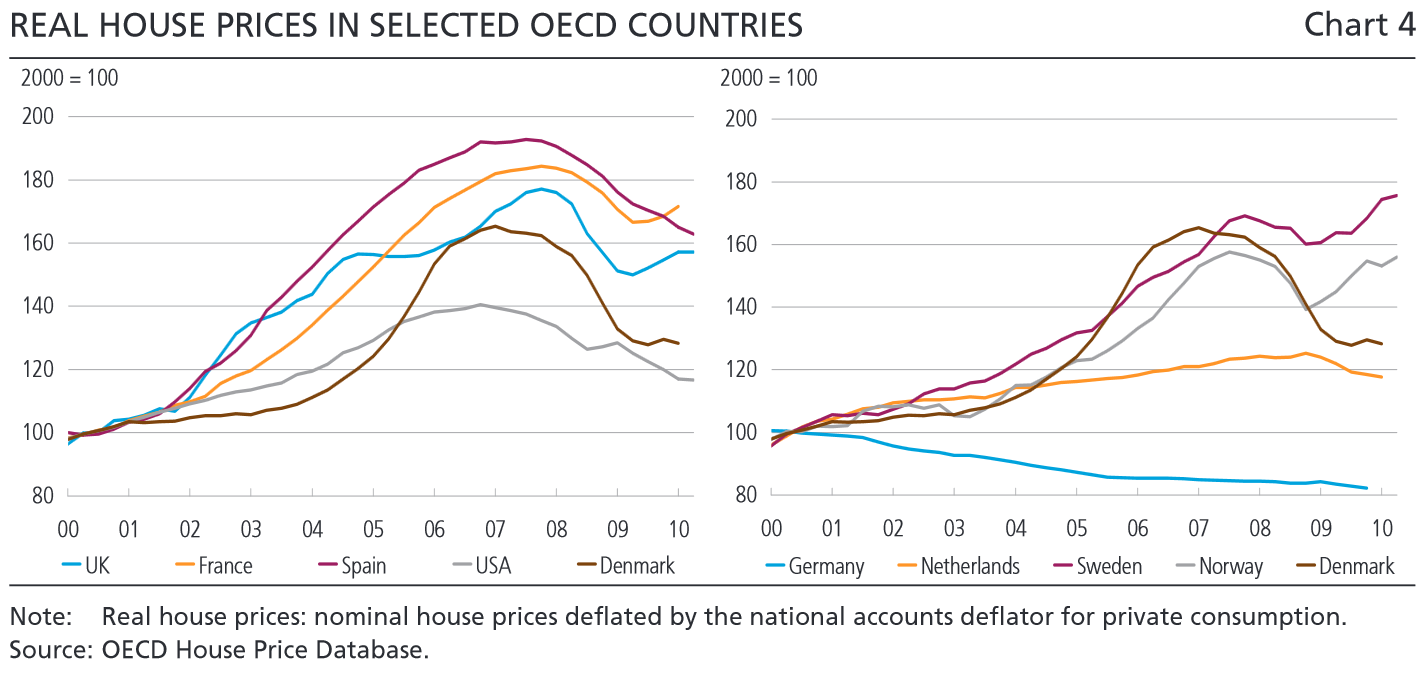
\includegraphics[width=0.9\textwidth]{../figures/intcomparison}
	\centering
	\caption{ Trends in real house prices in Denmark and selected OECD countries, 2000-2010 (2000 level = 100).  Taken from \citet[p. 50]{dam2011housing}}\label{dam}
\end{figure}

As shown in Figure \ref{dam}, although many economies experienced large increases in real house prices, Denmark's housing bubble was exceptionally volatile, characterized by a late, rapid increase quickly succeeded by a crash. The bulk of Denmark's housing boom and bust occurred in just four years, from 2005 to 2009. In contrast, the housing bubble in the United States (shown in the light gray line in the left panel of Figure \ref{dam}), though far bigger in absolute terms, was relatively protracted in comparison. As a consequence, local housing markets in Denmark saw year-to-year changes in housing prices that were, even by the standards of a globally economically volatile period, unusually large. This provides us with ample variation in the independent variable of interest.

Notably, Denmark's housing bubble was not merely a product of changes in the international business cycle. In fact, a majority of the housing bubble is typically attributed to national government policy. In 2002, the newly elected conservative government implemented a nominal freeze on property taxes, in effect cutting the real tax rate on property over time. The year after, the government introduced new loan types including deferred-amortisation loans which allowed homeowners to take out larger mortgage loans. In a study estimating the contribution of these domestic policies to the housing bubble, \citet[p. 62]{dam2011housing} conclude that ``two  thirds  of  the  additional  cyclical  fluctuations  that  accompanied  the  housing  bubble  can  be  attributed to the deferred-amortisation loans and the nominal tax freeze''.

The role of national government policy in driving the housing bubble is important, since it means voters have a reason to view house prices changes as a relevant informational source when evaluating government performance. The government's role in exacerbating the housing bubble was a politically salient issue in the aftermath of the Great Recession, so voters are likely to be aware of this link. However, although the policies exacerbating the housing bubble were implemented by the conservative government, which held office from 2001 to 2011, our argument does not cover only evaluations of the conservative government. If that were the case, evaluations of the government would be observationally indistinguishable from voters becoming more ideologically conservative, a plausible consequence of increases in housing wealth. In Section \ref{inference}, we exploit the change in incumbency in 2011-2015 to show that housing price changes affect support for the incumbent government per se, not merely support for a conservative government.

%Turning to the political context, the government in the entire period we investigate (2005-2015) consisted of two different parties. From 2001 to 2011 the Liberal party was in government along with the Conservative party, and from 2011 till 2015 the Social Democratic party and the Liberal party was in power.\footnote{An additional party, the Socialist party, was in government from 2011 to 2013, however, since this party left government before the election, it is excluded when looking at electoral support for the governing party. To get data on electoral support at the previous election, we also use some data from the 2001 election in which the Social Democratic party and the Liberal party was in power.} This change in party incumbency is useful, since it allows us to distinguish effects on incumbent government support from effects on macropartisanship. 

%Housing markets saw a boom followed by a bust in the period around the great recession. This had severe economic implications for wellbeing of both individual households’ and the overall state of the economy \citep{dam2011housing,ansell2014political}. Pairing the economic importance of the housing market with the fact that government regulations (or lack thereof) to a considerable extent influenced the severity of the market crash makes housing markets a particularly useful mean for voters to evaluate the incumbent government by. Furthermore, housing markets are not a monolithic national phenomenon, but vary substantially across geographical contexts, thereby providing voters with relevant local information by which to assess incumbents. 




%In this study we focus on how the housing bubble affected support for governing parties in Denmark. Denmark is privileged as a case for two reasons.

%The first is that Denmark had a very large housing bubble. As \citet[][49]{dam2011housing} explain concerning the housing bubble of the late 2000's ``developments in the Danish housing market in those years were unusually hectic, both in a historical and an international perspective''. This is also evident from Figure \ref{dam}, adapted from their paper. 

%\begin{figure}[htbp!]
%	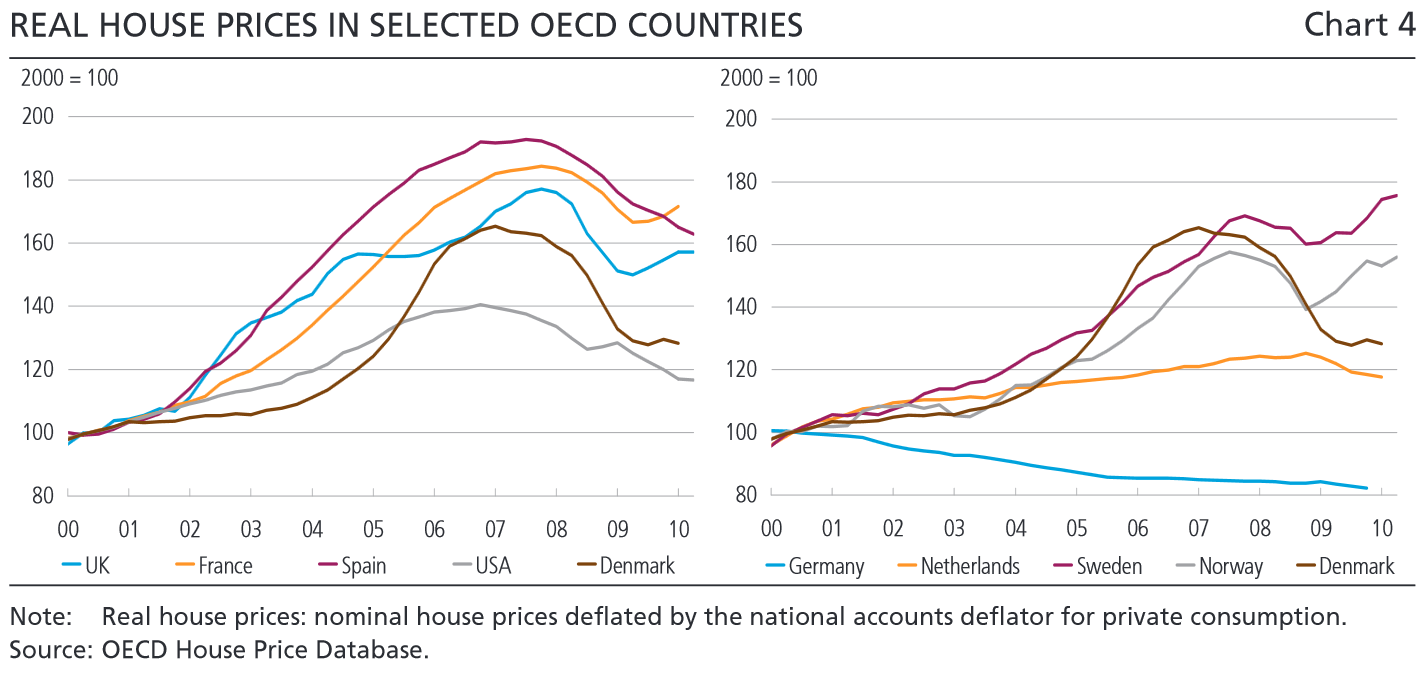
\includegraphics[width=0.9\textwidth]{../figures/intcomparison}
%	\centering
%	\caption{Taken from \citet[50]{dam2011housing}}\label{dam}
%\end{figure}

%The second reason we focus on Denmark, is that it is possible to obtain precise and comprehensive data on housing price changes, voting returns, and socio-economic controls at a very small geographic level. Existing approaches typically examine housing price returns at high levels of aggregation corresponding to either counties or entire states. In contrast, we observe housing price changes at the zip code level and voting returns and socio-economic controls at the precinct (i.e., polling place) level. This allows for much more precise measurements of the variables of interest and accordingly less attenuation of observed associations. We elaborate on the specifics of the data in the next section.



%\subsection{Identification strategy}
%
%
%We use a difference-in-difference approach controlling for other economic factors. 
%
%Use two different empirical approaches: Precinct level and Individual level data.

%\subsection{Identification strategy}

%In this article we want to identify the causal effect of recent changes in precinct level housing prices on electoral support for governing parties. Ideally, we would like to compare support for governing parties in the same district at a specific election across different levels of house-prices. As precincts were only assigned one change in housing prices per election, this is obviously not feasible. Instead, we need to construct a feasible observable counterfactual to a precinct with a specific change in housing prices, which we can use to difference out the effect of housing prices. 

%One way to do this is to simply compare incumbent support at different levels of housing price changes across elections and within precincts. Here the counterfactual for any given precinct is the incumbent support of an cross-elections average precinct. A key challenge to causal identification in this case is that certain structural features of precincts in which housing prices are likely to increase might make incumbents more popular. 

%We can begin to deal with this problem by examining the historical precinct-specific levels of incumbent support. As such, instead of simply using an average of all precincts as our counterfactual, we can use the average for the individual precinct. Comparing incumbent support within precincts and across different levels of housing prices. This takes into account that certain precincts might be historically more inclined to support incumbents and have increasing housing prices. However, it does not take into account that when housing prices are relatively high in a district in a particular election, it is also likely to be high in other precincts as well. This is problematic if incumbents do systematically better or worse, in general, when housing prices are doing well.

%To address this problem, we can examine levels of incumbents support, not just relative to the precincts history, but also relative to the level of incumbent support across districts. In this case, our counterfactual for any given precinct is the electoral support that governing parties typically obtain in that precinct, plus or minus the overall change in electoral support for governing parties across all precincts. This gives us a difference-in-differences approach to identifying the effect of housing prices. As such, we look at differences within elections in differences between the individual precincts typical and actual outcome.

%The difference-in-differences approach makes it possible to compare with a very reasonable counterfactual situation -- what is the typical incumbent support we could expect in a precinct given the overall popularity of the incumbent. However, since the the governing parties change from election to election, and since the priorities of the same parties might change from election to election, different types of precincts might prefer government parties at  different elections. This poses a challenge to causal identification. As such,  these changes in election and precinct-specific preferences might not be the same across types of precincts which experience increasing and decreasing in housing prices. We cannot completely deal with this problem: As mentioned in the beginning of this section, we have only one piece of information on the assigned housing price change for a precinct at an individual election. However, we can create an even more appropriate counter-factual by taking into account how precincts of a specific type do at specific elections.

%First, we can take the precincts economic status into account. That is, how the incumbent scores on the four structural variables mentioned above: income, wealth, employment and benefits. In this case our counterfactual for any precinct will be be the typical incumbent support we would expect a precinct to have given how popular the incumbent is at this specific election in precincts with a similar economic make-up.

%Second, we can take the precincts geographical location into account. Specifically, we can look at what municipality,  the smallest local administrative unit in Denmark, the municipality is located in. In this case our counterfactual for any precinct will be be the typical incumbent support we would expect a precinct to have given how popular the incumbent is at this specific election in precincts in the same municipality.

%This counter-factual can be expressed using the following linear equation.

%\begin{equation}
%y_{it}= \delta houseprices_{it} + \pi_i + year_{it} + \epsilon_{it}
%\end{equation}

%Where $y_{it}$ is incumbent support at election $t$ in precinct $i$ and $houseprices_{it}$ is year-over-year changes in housing prices. $\delta$ is the coefficient of interest, as it represents the effect of housing prices on incumbent support.  $\pi_i$ represent precinct fixed-effects and $\epsilon_{it}$ is an error term. $year_{it}$ is a year and precinct specific term, which signifies how much more or less popular, we would expect the incumbent to be in an individual precinct at a specific election, given its geographical location and economic status. It is defined as

%\begin{equation}
%year_{it}=\mathbf{X_i\beta_t + Z_i\gamma_t}
%\end{equation}

%$ \mathbf{X_i}$ is a vector of the four economic variables and $\mathbf{\beta_t}$ is a vector of coefficients attached to these variables, which specify the relationship between these variables and incumbent popularity at time $t$. $\mathbf{Z_i}$ is a vector of 98 dummy variables indicating which of 98 municipalities the precinct lies within. $\mathbf{\gamma_t}$ is a vector of coefficients attached to these dummy variables, which specify the cross-precinct municipal average of incumbent popularity at time $t$.


%difference in difference - control for other economic conditions. Problem is - however way better than earlier...

%Limitation
%Before moving on it is important to note an important limitation of the present study. What we find is an aggregate level correlation. As such, we do not know whether voters punish and reward the government for the quality of local housing prices  because (1) their own house loses some of its value (egotropic), (2) they fear for the future of their community (geotropic) or (3) they infer something about the state of the national economy from their local area (sociotropic). The aggregate-level data used in this study cannot distinguish between these competing models of individual-level cognition. However, given the state of the extant literature on housing prices and the effects of the local economy, simply establishing an effect and describing how this effect varies is substantial step forward. 

\section{Precinct-level evidence}\label{precinctlevel}
We begin our exploration of the relationship between the state of local housing markets and incumbent support by looking at precinct-level election returns in Danish Parliamentary elections between 2005 and 2015. In particular, we match electoral support for parties in government in these precincts with change in the price of all house sales sold in and around the precincts, examining the extent to which local housing prices and local electoral support for government parties go hand in hand.

\subsection{Data sources and indicators}
The key dependent variable in our study is \textit{percent of votes cast for government parties} in each voting precinct. Each voting precinct corresponds to a single polling place and is this the smallest unit at which voting returns can be observed in Danish elections. We measure this for all precincts in four elections:  2005, 2007, 2011 and 2015. There are roughly 1,400 precincts, each precinct consisting of about 3,000 eligible voters on average and covering an average area of 30 square kilometers. A number of precincts are redistricted between each election. This is problematic, as we want to use  the precincts as part of a panel data set. There are two ways to deal with this. We can drop precincts as their geographical boundaries get altered. This would mean dropping roughly 15 pct. of the data on the dependent variable. The other option is to fix the precincts geographical boundaries at one reference election (i.e. 2015), and then recalculate vote returns in any changed precincts, so they match up with precincts in the reference election. Since there are a lot of minor changes in geographical boundaries from election to election, but only a few major changes, we opt for the latter, which allows us to keep these slightly altered districts in the analysis.\footnote{For details of how returns from the redistricted precincts are calculated, see Søren Risbjerg Thomsen's research note at \texttt{\href{http://bit.ly/205OlPi}{bit.ly/205OlPi}}.  We use 2015 as a reference elections}. 

The key independent variable is \textit{change in local housing prices}. We obtain housing price data from The Danish Mortgage Banks' Federation (\textit{Realkreditforeningen}), which publishes quarterly data on the average price per square meter of all sales at the zip code level.\footnote{Available at \texttt{\href{http://statistik.realkreditforeningen.dk/}{statistik.realkreditforeningen.dk}}.} For each election, we calculate change in housing prices as the percentage change in the price of houses sold in the quarter of the election compared to the same quarter one year before. 

Zip codes are a substantively interesting level of aggregation when it comes to the price of housing, as it is the level at which house prices are most often reported in Denmark (cf. the fact they are published by The Danish Mortgage Banks' Federation). However, since the dependent variable is measured at the precinct level, merging these observations is not trivial. The easiest solution would be to extract the zip code of the address of each polling place and link the polling place to housing prices in that zip code. Unfortunately, full addresses are not available for all polling places. Instead, we use a three-stage approach to linking polling places to zip codes. First, we extract the street address and higher-level voting district of each polling place (the full resulting string is of the format `Streetname streetnumber, City, Denmark'). Second, we pass this string to the Google Maps API, which geocodes the string and returns latitude-longitude coordinates.\footnote{Available at \texttt{\href{https://developers.google.com/maps/documentation/geocoding/intro}{developers.google.com/maps/documentation/geocoding/intro}}.} Third and last, we pass these coordinates to the Danish Addresses Web API (DAWA), a public service provided by the Danish Geodata Agency.\footnote{Available at \texttt{\href{http://dawa.aws.dk/}{dawa.aws.dk}}.} The DAWA returns the zip code for each address, allowing us to link the two sources of data. %It is important to note that statistically speaking, precincts are therefore nested inside zip codes; we take this into account by clustering the standard errors on the precinct-level in our analysis.

We examine changes in prices rather than price levels. This is in part because previous economic voting literature, to the extent that it has looked at prices, have also focused on changes (i.e. inflation) rather than levels \citep[cf.][]{kramer1971short}, and in part because it seems likely that changes in housing prices will be more salient for voters than levels. As such, changes in housing price will mean either very short or very long turnaround time, as sellers and buyers try to adjust to the new prices, leaving visible traces of these changes in the voters immediate context -- such as the number of for sale signs, and the speed at which old neighbors are exchanged for new ones.

In addition to the main independent variable, we measure both the unemployment rate and median income at the zip-code level. We also measure the population density ($log(inhabitants/km^2)$) of the municipality in which the precinct is located. These are all population based measures calculated from national registers provided by Statistics Denmark.


\subsection{Estimating the average effect of housing prices}
In table \ref{predv}  we report estimates from a set of linear regression of electoral support for governing parties using changes in local housing prices as the primary independent variable. For all models we use robust standard errors clustered at the precinct-level. In the first column we present a simple linear regression between electoral support and changes in housing prices. In the second column we add year fixed effects, holding trends in incumbent support and rates of housing price changes constant. In column 3 we add precinct fixed effects. In effect, model 3 evaluates if differences in within-precinct changes in housing prices is related to changes in support. This setup hold averages rates of change constant, and thus effectively eliminate confounding by time-invariant circumstances at the precinct level that may lead to different trajectories in housing prices over time. In column 4 we we include the unemployment rate and median income as controls for the trend of the state of the economy in the precinct.



\begin{table}[htbp]\centering
\def\sym#1{\ifmmode^{#1}\else\(^{#1}\)\fi}
\caption{Estimated effects of house prices on electoral support for governing parties.} \label{predv}
\begin{tabular}{l*{4}{c}}
\hline\hline
                    &\multicolumn{1}{c}{(1)}        &\multicolumn{1}{c}{(2)}        &\multicolumn{1}{c}{(3)}        &\multicolumn{1}{c}{(4)}        \\
\hline
$\Delta$ housing price&       0.104\sym{**}&       0.048\sym{**}&       0.053\sym{**}&       0.030\sym{**}\\
                    &     (0.008)        &     (0.007)        &     (0.008)        &     (0.007)        \\
[1em]
Unemployment rate   &                    &                    &                    &      -1.898\sym{**}\\
                    &                    &                    &                    &     (0.221)        \\
[1em]
Log(Median income)  &                    &                    &                    &      -0.891\sym{**}\\
                    &                    &                    &                    &     (0.064)        \\
[1em]
\hline Year FE      &                    &$\checkmark$        &$\checkmark$        &$\checkmark$        \\
[1em]
Precinct FE         &                    &                    &$\checkmark$        &$\checkmark$        \\
\hline
Observations        &        4193        &        4193        &        4193        &        4173        \\
RMSE                &       8.403        &       6.748        &       5.713        &       5.321        \\
\hline\hline
\multicolumn{5}{l}{\footnotesize Standard errors in parentheses}\\
\multicolumn{5}{l}{\footnotesize \sym{*} \(p<0.05\), \sym{**} \(p<0.01\)}\\
\end{tabular}
\end{table}



As can be seen from table \ref{predv}, there is a statistically significant and positive coefficient attached to changes in housing prices, indicating that a larger fraction of the electorate casts their vote for governing parties in precincts where housing prices are increasing. In the most demanding specification the coefficient is 0.03, the implication being that if the price of housing sold in a precinct's zip-code in the last quarter before the election is twice that of the housing sold in the same quarter the year before, electoral support for  governing parties in this precinct will increase with roughly 3 percentage points.

Unsurprisingly, the effect is larger in the models which use fewer controls --  the effect size drops from 0.1 to 0.05 when introducing the economic controls, and drops an additional 0.02 when introducing the time and precinct fixed effects. This seems to suggest that using a difference-in-difference approach and detailed information about other aspects of the local economy is, in fact, important when identifying the effect of local housing prices on incumbent support.


\begin{table}[htbp]\centering
	\def\sym#1{\ifmmode^{#1}\else\(^{#1}\)\fi}
	\caption{Assesing the Robustness of the Precinct-level Evidence} \label{robustness}
	\begin{tabular}{l*{4}{c}}
		\hline\hline
		&\multicolumn{1}{c}{(1)}        &\multicolumn{1}{c}{(2)}        &\multicolumn{1}{c}{(3)}        &\multicolumn{1}{c}{(4)}        \\
\hline
$\Delta$ housing price (2 years)&       0.129\sym{**}&       0.037\sym{**}&       0.022\sym{**}&       0.020\sym{**}\\
&     (0.007)        &     (0.007)        &     (0.007)        &     (0.007)        \\
[1em]
$\Delta$ housing price (FD controls)&       0.104\sym{**}&       0.073\sym{**}&       0.086\sym{**}&       0.058\sym{**}\\
&     (0.008)        &     (0.008)        &     (0.009)        &     (0.008)        \\
[1em]
$\Delta$ housing price (FD DV)&       0.037\sym{**}&       0.034\sym{**}&       0.052\sym{**}&       0.019\sym{**}\\
&     (0.004)        &     (0.004)        &     (0.005)        &     (0.004)        \\
[1em]
$\Delta$ housing price (negative)&      -0.081\sym{***}&      -0.072\sym{***}&      -0.057\sym{**} &      -0.030         \\
&     (0.022)         &     (0.017)         &     (0.019)         &     (0.019)         \\
[1em]
$\Delta$ housing price (positive)&       0.116\sym{***}&       0.045\sym{***}&       0.031\sym{**} &       0.029\sym{*}  \\
&     (0.012)         &     (0.011)         &     (0.011)         &     (0.011)         \\
[1em]
\hline Economic controls  &                    & $\checkmark$                    &$\checkmark$        &$\checkmark$        \\
[1em]
Precinct FE  &                    &                    &$\checkmark$        &$\checkmark$        \\
[1em]
Year FE             &                    &                    &                    &$\checkmark$        \\
\hline\hline
\multicolumn{5}{l}{\footnotesize Standard errors in parentheses}\\
\multicolumn{5}{l}{\footnotesize \sym{*} \(p<0.05\), \sym{**} \(p<0.01\)}\\
\end{tabular}
\end{table}

How robust are these results? In table \ref{robustness} we try to reanalyze the models above in different ways, to get a more complete picture of the statistical evidence for (or against) the importance of local housing markets for incumbent support. 

We begin by looking at whether the chosen time period, i.e. year-over-year changes, is important. To do so we reestimate the models from table \ref{predv} using the change in housing prices over two years rather than one. The results are fairly similar using this measure of more long run changes in housing prices, however, the estimated effects tend to be smaller than what we found above. This fits nicely with previous work showing that voters are, by and large, myopic when it comes to relating economic indicators to incumbent support \citep{healy2009myopic,healy2014substituting}. 

As mentioned above, we use changes in house prices rather than levels. However, in our models we control for the level of income and the level of unemployment. One could imagine, that this means that we fail to capture something important about how the economic status of the precinct is changing, which could, in turn, be driving our results. To examine whether this is the case, we re-estimate the different models using first-differenced (FD) controls. As can be seen in the fourth row of table \ref{robustness}, this does not change the results substantially, if anything, the estimated effects of local housing prices doubles in size. We also estimated a set of complete change models, using an FD dependent variable as well. The estimates from these models are reported in the fourth row of the table. The estimated effect size of housing prices in the completely differenced model is somewhat smaller than what was identified in table \ref{predv}, but it remains statistically significant.

As a final robustness test we split the housing price variable in two, creating one variable which measures the size of positive changes, which is zero if there is a negative change, and one variable which measures the size of negative changes, which is zero if there is a positive change. This makes it possible to study the effect of increases and decreases in housing prices separately. We report the result of these analyses in the two last rows of table \ref{robustness}. Interestingly, the effect of negative changes an positive changes do not seem to differ - they are roughly 0.03. This is both important and somewhat surprising. Important, because it suggests that incumbent politicians are not only rewarded for the boom or punished for the bust. Instead, voters seem to first reward governing politicians when house prices are on the rise, and then punish them when they fall. Somewhat surprising, because much previous research have found that voters respond more strongly to negative economic conditions \citep[e.g.][]{bloom1975voter,headrick1991attention,soroka2014negativity}.

Taken together, these analyses suggest that there is a robust, positive effect of local housing prices on support for governing parties.

\subsection{Placebo test}
Next, we look at whether  governing parties were already getting more popular in places where housing prices would eventually increase and getting less popular in places where housing prices would eventually decrease. To do this we estimate the same type of models as in table \ref{predv}, using support for the governing party at the last election as the dependent variable -- the lag of the dependent variable. We plot the estimated effects of housing prices on the lag of the dependent variable, as well as on the dependent variable, in figure \ref{placebo}. As can be seen from this figure there is an significant effect of housing prices on the lagged dependent variable in the less restrictive models, however, in the final model, the estimated effect of housing prices is 0.005 -- less than a sixth of the estimate in the corresponding model in table \ref{predv} -- and statistically insignificant. This is important, because a key assumption underlying the difference-in-difference design employed here is that prior trends in the dependent variable are uncorrelated with the independent variable  (i.e. the parallel trends assumption). This analysis seems to suggest that there was no such correlation.

\begin{figure}[htbp!]
	\includegraphics[width=0.9\textwidth]{../figures/lagdv.eps}
	\centering
	\caption{Effects of Housing Prices on support for governing party at the present election (t) and the last election (t-1) with 90  and 95 pct. Confidence Intervals}\label{placebo}
\end{figure}



\section{Individual-level evidence}\label{individuallevel}
We continue our study of how local housing markets shape incumbent support by tracking a representative sample of Danish citizens in a two wave panel survey collected between 2002 and 2011. We link the survey respondents to the prices of housing sold in their residential context using the national Danish registers. The registers contain very detailed information about all individuals legally residing in Denmark, including the exact geographical location of their residence, the price of any real estate they sell, and a range of other socio-demographic characteristics \citep{thygesen2011introduction}. This makes it possible to calculate the distance between the individuals in the survey and all other individuals in Denmark and, in turn, the distance to any individuals who are selling their home. 
 
 While it is always desirable to try and replicate findings using a different methodology and a different set of data, linking individual level data to these detailed registers has some advantages over the precinct-level data used above. The flexibility and detail of the Danish registers makes it possible to look at multiple levels of aggregation -- not just official levels of aggregation, such as zip codes. This makes it possible to eliminate concerns related to the modifiable area unit problem (MAUP), in that we can rule out that the findings are tied to a specific way of geographically aggregating housing prices. Further, and more important for our theoretical argument, we can also link housing prices to individual level variables such as attitudes or home ownership, and use these variables to rule out alternative explanations and explore individual-level moderators of the housing price effects.




\subsection{Data sources and indicators}
Our independent variable is once again year-over-year changes in housing prices in the residential context of the respondent. We measure the change by comparing the price of housing sold in the quarter prior to the data collection and the price of housing sold in the same quarter a year earlier. Unlike for the precinct-level data  we do not have data on prices per square meter. This makes the individual-level housing price change variable more sensitive to random variation in the types of housing put up for sale in the two time periods we compare. As such, some of the changes from year to year might be due to the fact that larger houses were put up for sale in one year. To take this, as well as other structural differences in the type of housing put up for sale, into account we divide the sales price of each unit of housing by its public valuation, before calculating the year-over-year change.\footnote{The Danish government makes a conservative estimate of the price of all housing in Denmark every two years which is used to calculate property taxes. The public evaluation was constant across the time periods we use to estimate housing price changes.} 

We estimate the changes in housing prices within each survey respondent's residential context, measuring this context  in three different ways. First, and similar to what we did for the precinct-level data, we use the respondents zip-code, comparing housing sold within the same zip code a year apart. Second, we look at the prices of the 20 or 40 units of housing sold closest to the respondents own home, comparing the prices of housing sold in the immediate proximity of the respondent to that of housing sold one year earlier. Third, we look at the price of housing sold within a fixed radius of 1000 or 1500 meters of the respondent. These latter ways of defining the respondents residential contexts have the benefit of being centered on the respondent, alleviating the problem that the context of a respondent living far from the centroid of one zip-code might be better represented by an adjoining zip-code. Note also that these latter two types of residential context differ in important ways -- whereas the first method takes number of sales as fixed, but varies the geographical dispersion of these sales, the second method holds geographical dispersion fixed, but varies the number of sales. Since it is not obvious which of the three ways of measuring the states local housing market is preferable, we will use them all in the analysis below.\footnote{To do this we use all housing sales registered in the national register EJSA, which do not fall into one or more of the following categories: (1) Sales of part of a house or apartment (10 pct. of all sales). (2) Sales of commercial real estate (9 pct). (3) Sales of apartments or houses valued at more than DKK 10 million (0.2 pct. of all sales) (4) Sales with what `Statistics Denmark' calls an irregular price (i.e. if the sales price is more than three times the valuation or less than forty percent of the valuation, 6 pct. of all sales).}

To get at support for governing parties at the individual level we utilize a two-wave panel survey, constructed by re-interviewing respondents who had participated in the Danish Version of the European Social Survey (ESS);  a nationally representative survey conducted regularly in most European countries. All in all 1,745 people were re-interviewed in the winter of 2011-12, with some of these having been interviewed for the first time in 2008/9, some in 2004/5 and some in 2002/3 -- corresponding to rounds four, two and one of the ESS. 

The respondents in the ESS in Denmark are randomly sampled from the national civil registry, and therefore the civil registration numbers were retained by the data collection agency. This made it possible to identify the respondents for a second interview, and made it possible to link the respondents to the national registers. From the survey, we use the following question: ``What party did you vote for at the last parliamentary election?'' Respondents were presented with all the parties which ran in the previous election. For the analyses we create a dummy variable indicating whether the respondent voted for a party in government at the time of the election. 

In addition to these central variables, we also use a number of supporting variables in the analysis for statistical control, interaction analyses and placebo tests. As controls, we include unemployment and income both for the individual respondent and in the respondents immediate context. We present the remaining variables as we introduce them in the analysis.

\subsection{Average effect}
In table \ref{inddv}  we report estimates from a set of linear probability models (LPM), setting the probability of voting for for a party in government as a function of changes in local housing prices. We estimate the models using a linear regression with fixed effects for the respondent, and fixed effect for which of the four different survey rounds the respondent is participating  (ESS round one, two, four or the re-interview). All models include controls for the average income and unemployment rate in the respondents context, as well as indicators of the respondent's own income and whether someone in the household is unemployed. As such, we end up with a difference-in-difference model which controls for trends in the economic situation -- however, unlike for the precinct level data we can now control for trends in both the individuals personal economy and for the economy of the larger context. We use robust standard errors, clustered at the individual level.

All models include the same set of variables, but they differ in how the contextual variables are operationalized. In column one we present a model where housing price change is calculated based on the 20 closest sales (cf. above), and the other contextual variables -- average income and unemployment rate -- is measured within a 500 meter radius of the respondent. In column two we use the 40 closest sales, but leaves the remaining variables operationalized as in column one. In column three and four we operationalize all contextual variables, sales, unemployment rate and average income, as 1000 and 1500 meter radii around the respondent. Finally, in column five, we examine sales at the level of zip-codes, but the other contextual variables are calculated based on people within a 1500 meter radii around the respondent.

\begin{table}[htbp]\centering
\def\sym#1{\ifmmode^{#1}\else\(^{#1}\)\fi}
\caption{Linear Regression of Voting for Governing party } \label{inddv}
\begin{tabular}{l*{5}{c}}
\hline\hline
                    &\multicolumn{1}{c}{20 Closest}&\multicolumn{1}{c}{40 Closest}&\multicolumn{1}{c}{1000 metres}&\multicolumn{1}{c}{1500 metres}&\multicolumn{1}{c}{Zip code}\\
\hline
$\Delta$ housing prices&       0.035       &       0.056       &       0.064       &       0.114\sym{*}&       0.063       \\
                    &     (0.036)       &     (0.044)       &     (0.052)       &     (0.051)       &     (0.056)       \\
[1em]
Unemployment rate   &       0.052       &       0.056       &      -0.439       &       0.755       &       0.796\sym{+}\\
                    &     (0.290)       &     (0.289)       &     (0.627)       &     (0.575)       &     (0.422)       \\
[1em]
Average income      &      -0.004       &      -0.004       &      -0.005       &      -0.005       &      -0.006       \\
                    &     (0.003)       &     (0.003)       &     (0.007)       &     (0.007)       &     (0.006)       \\
[1em]
Personal income     &      -0.000       &      -0.000       &      -0.000       &      -0.000       &      -0.000       \\
                    &     (0.000)       &     (0.000)       &     (0.001)       &     (0.001)       &     (0.000)       \\
[1em]
Unnemployed (household)&      -0.032       &      -0.033       &      -0.066       &      -0.048       &      -0.034       \\
                    &     (0.035)       &     (0.035)       &     (0.043)       &     (0.040)       &     (0.036)       \\
[1em]
\hline  Round FE    &         Yes       &         Yes       &         Yes       &         Yes       &         Yes       \\
[1em]
Individual FE            &         Yes       &         Yes       &         Yes       &         Yes       &         Yes       \\
\hline
Observations        &        3479       &        3479       &        2790       &        2992       &        3384       \\
\hline\hline
\multicolumn{6}{l}{\footnotesize Standard errors in parentheses}\\
\multicolumn{6}{l}{\footnotesize \sym{+} \(p<0.1\), \sym{*} \(p<0.05\)}\\
\end{tabular}
\end{table}


The estimated coefficients are positive across the different models, although the size of the coefficient varies somewhat, going from 0.04 to 0.11. The effect is only statistically significantly different from zero in one of the five specification -- the one which looks at the 1500 meter context. 

One interpretation of these findings is that the lack of systematic statistically significant coefficients suggests that there is no effect of housing price changes. Such an interpretation fails to take into account, that the coefficients  estimated for the individual-level data is actually consistent with what we found in the precinct-level data. To see this figure \ref{comparison} plots the estimated effect of housing prices estimated for the individual-level data in table \ref{inddv}  and for the precinct-level data in table \ref{predv}.

\begin{figure}[htbp!]
	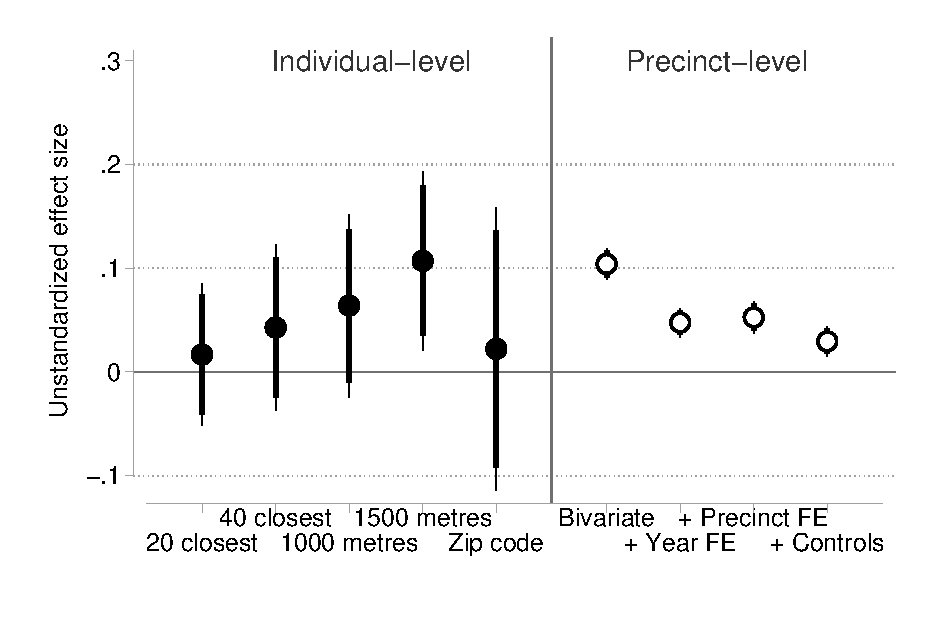
\includegraphics[width=0.9\textwidth]{../figures/comparison.eps}
	\centering
	\caption{Effects of Housing Prices across levels of analysis with 90  and 95 pct. Confidence Intervals}\label{comparison}
\end{figure}

As can bee seen from the figure, the effect sizes are pretty similar across levels of analysis - if anything they are larger for the individual level data. Put differently, a one reason that we cannot identify statistically significant effects in the individual level data is that that the housing price effects are not as precisely estimated. This interpretation, that the estimated coefficients do not represent a null-effect, but rather an imprecisely estimated effect, is further corroborated in the next section when we do find a statistically significant effect for a sub-group which should be especially attuned to hosing prices.

\subsection{Self-interest, Ideology or Inference}\label{inference}

In a recent study \cite{ansell2014political} finds that people become more right-wing, , in the sense of being less supportive of redistribution, when the price of their home increases. Since their is a Conservative government in much of the period we study (2001-2011), it is interesting to ask whether our results are driven by voters becoming more conservative as local housing prices increase. 

To examine this we run the same models as in table \ref{inddv} substituting incumbent support for ideological self placement on a ten point scale going from left to right as the dependent variable. For the analysis we rescale the variable to go between zero and one. We report the estimated effects of changes in housing prices on ideological orientation in figure \ref{ideology}. For comparison, we also plot the effects on incumbent support. As can be seen from this figure there is no discernible effect on ideology, the estimated effects being very close to zero in all models.


\begin{figure}[htbp!]
	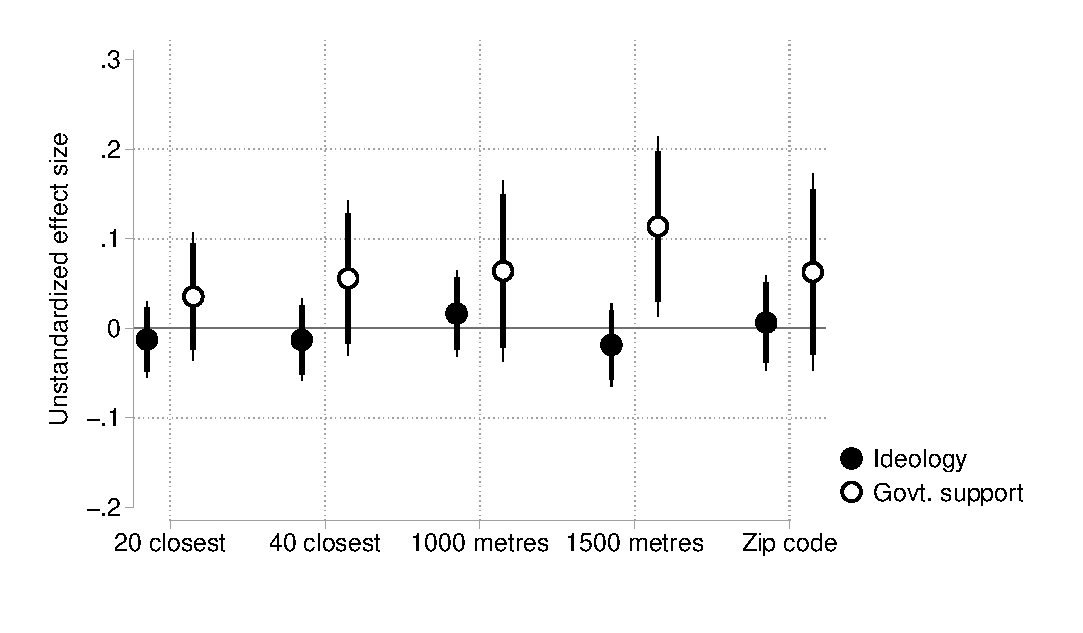
\includegraphics[width=0.9\textwidth]{../figures/ideology.eps}
	\centering
	\caption{Effects of Housing Prices on Ideological Orientation and Support for Governing Parties with 90  and 95 pct. Confidence Intervals}\label{ideology}
\end{figure}

A related question is whether voters reaction to housing prices is shaped by self-interest. That is, are people responsive to changes local housing prices because they believe these changes indicate that their own home will be worth more. 

To examine this we re-estimated the different models, including an interaction between whether voters owned their own home (i.e. rented), and changes in housing prices. We then derived the estimated marginal effects of changes in housing prices for home owners and others. These marginal effects are plotted in figure \ref{homeown}.

The results are a bit mixed with some models showing effects to be slightly larger for home owners, and other models showing no difference. On balance, however, there does not seem to be any systematic evidence for the conjecture that it is only home owners that are affected by changes in housing prices.

\begin{figure}[htbp!]
	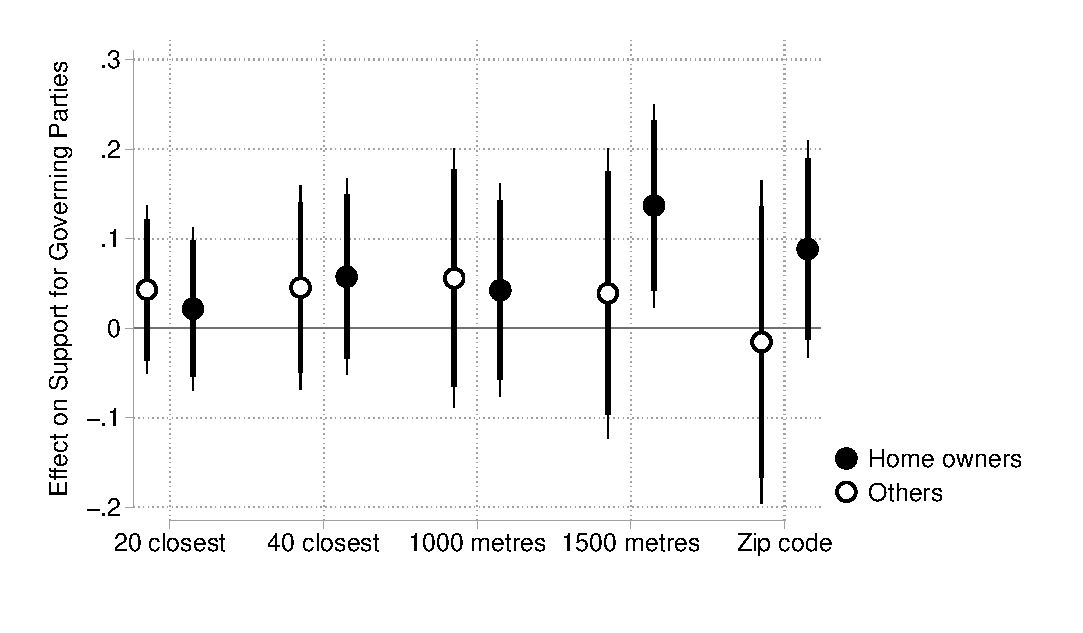
\includegraphics[width=0.9\textwidth]{../figures/homeown.eps}
	\centering
	\caption{Effects of Housing Prices for those who own their home and those who do not with 90  and 95 pct. Confidence Intervals}\label{homeown}
\end{figure}

Why might people who do not own a house be affected by changes in local housing prices? One reason, which we alluded to in the beginning of the paper, is that local housing markets serve as a signal of incumbents competence. As such, even though you do not own your home, you might infer from a booming local housing market, that incumbent politicians are doing a good job keeping your local community economically well off.

If voters are in fact using local housing markets as a signal of incumbent quality, we would expect those who are more finely attuned to this signal to be more affected by local housing prices.

To test this, we construct a variable from the national registers, which measures whether the respondent was likely to be attuned to the housing market. In particular, we measure whether the respondent moved within two years before or after being surveyed. To take into account that respondents who moved within one year of being surveyed were probably more attuned than those who moved within two years, we gave respondents a score of one if they moved out the day after or before being surveyed, and then we let the score steadily declines until after two years it was zero (i.e. if you moved within exactly one year you had a score of 0.5).

In figure \ref{move} we derive marginal effects from these models for those who have not moved in two years (i.e. scores 0) and the effect for those who move day before or after the survey (ie. scores 1). The estimated effect of housing prices is very large for those respondents who are on the cusp of moving, and, importantly, is statistically significant in all specifications ($p<.05$ for all models except the one for zip-codes for which $p<.1$). The marginal effects for the movers are also significantly larger than the effects for the stayers ($p<0.05$) in four out of the five specifications.

\begin{figure}[htbp!]
	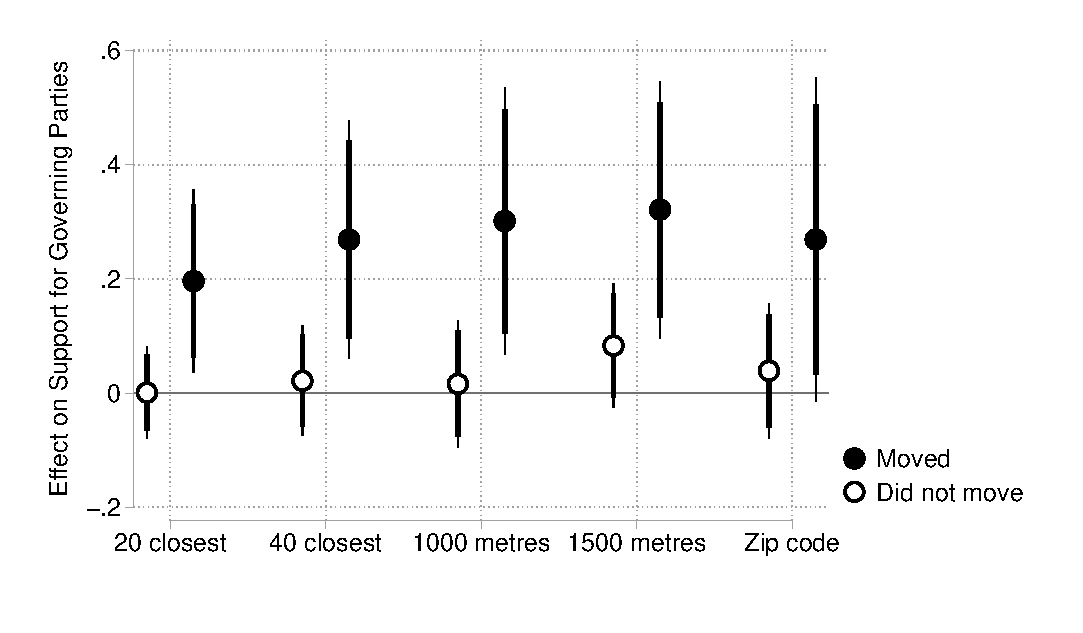
\includegraphics[width=0.9\textwidth]{../figures/moving.eps}
	\centering
	\caption{Effects of Changes in Housing Prices for those who had just or were going to move and those who did not with 90 and 95 pct. Confidence Intervals}\label{move}
\end{figure}

Taken together, these analyses suggest that the housing price effect is not related to ideology or `simple' self-interest. Instead, voters the importance of local housing prices seems to be that they, to the extent that voters are attuned to the local housing market, gives present voters with a signal of the incumbent competence in handling the economy.



\section{Conclusion}
Housing prices tell you something fundamental about the economic situation of a local community. Just like unemployment or local economic growth, housing prices shape the experience and the fate of a community. Therefore housing prices might play an important role in politics. In this article we wanted to examine one possible political effect of changes in local housing prices – that on support for governing parties in Denmark. Using precinct-level data on four Danish Parliamentary elections bookended by a dramatic economic bubble in real-estate prices, we found a positive effect of changes in housing prices on electoral support. Our results suggest that as housing prices increase, so does electoral support for governing parties. Linking a two-wave panel survey of Danish voters to the national Danish registers, we then replicated this finding, identifying a comparable effect. Analyzing the panel data in more detail, we found that the effect of housing prices was especially pronounced among those who were more likely to be attuned to the state of their local housing market. 

Though the data used in this study is a clear improvement compared to those in earlier studies, its major shortcoming is that the data is nonetheless observational. In the absence of fully or quasi-experimental variation in housing prices, we cannot be sure that the estimated effects are not confounded by unobserved heterogeneity. This concern remains even though we apply highly stringent tests to the effect estimate. Hence, a promising avenue for future research is to identify settings with plausibly exogenous variation. 

What implications do these findings have? First, politicians should care about housing prices and the policies that influence them. If not they risk facing electoral retribution. Further, since voters are sensitive to  local differences in housing prices, politicians cannot simply be attentive to housing prices as a whole, but have to worry about the geographic distribution of any housing booms and busts \citep[cf.][11]{ferejohn1986incumbent}. This aspect, that voters care about local economic conditions, is especially interesting in light of the fact that most studies of the electoral effects of the economy have focused on the national economy or, to a lesser extent, personal economic conditions \citep[290]{healy2013retrospective}. 



% LEFTOVERS

 %First of all, just like we can learn about political business cycles from studying voter myopia \citep{healy2014substituting,tufte1980political}, or learn about the prevalence of disaster relief vis-à-vis disaster prevention by looking at how voters reward spending on one or the other \citep{healy2009myopic,ashworth2012electoral}, studying how voters react to housing bubbles tells us something about the political antecedents of these bubbles. Specifically, it highlights the incentives reelection-minded politicians face when developing policies which influence the formation of economic bubbles.

%Housing prices tell you something fundamental about the economic situation of  a local community. Just like unemployment or local economic growth, housing prices shape the experience and the fate of a community. Therefore housing prices might play an important role in politics. In this article we wanted to examine one possible political effect of changes in local housing prices -- that on support for governing parties in Denmark. Using precinct-level data on four Danish Parliamentary elections bookended by a dramatic economic bubble in real-estate prices, we found a positive effect of changes in housing prices on electoral support. Our results suggest that as housing prices increase, so does electoral support for governing parties. Does this reflect a causal relationship? While it is notoriously hard to know for sure using observational data, we have shown suggestive evidence that the effect is in fact causal. We have also shown that there is substantial heterogeneity in the effect. Specifically, negative changes seem to have larger effects than positive changes, and changes in areas where prices are more volatile seem to have larger effects than changes in areas, in which prices are less volatile.

%The observed heterogeneities in the effects of housing prices lend themselves easily to conclusions about the motivations of voters punishing or rewarding government parties. Specifically, the stronger observed effect for negative changes over positive ones might lead one to conclude that voters suffer from negativity bias. Conversely, the stronger observed effect in high-volatility areas suggests that voters attempt to parse out the `policy-elasticity' of observed housing price changes. 

%Both of these explanations may account for the effects observed here, but caution is warranted when inferring individual-level motivations from aggregate-level effects. Instead, we would argue that the main implications of these findings is not about the rationality of individual voters, but rather the incentives faced by governments. Specifically, the results of this study suggest that even for narrowly office-seeking, myopic governments would not benefit from policies that inflate housing bubbles. Regardless of their motivations, voters systematically react strongly to bubble-like housing price volatility and punish downturns significantly more than they reward upturns. The evidence thus implies that the expected ballot box gains of inflating housing bubbles are negative.






.





\clearpage

\singlespacing

\bibliographystyle{apa}
\bibliography{library}

%\newpage

%\section*{Supplementary materials}

%\subsection*{S1:Descriptive statistics}

%Table of descriptive statistics

%\newpage

%\subsection*{S2: Common trends in precinct-level data}
%In table \ref{prelagdv} we look at whether housing prices can predict changes in support for governing parties in the last period. 


%\begin{table}[htbp]\centering
\def\sym#1{\ifmmode^{#1}\else\(^{#1}\)\fi}
\caption{Estimated effects of house prices on electoral support for governing parties at t-1.} \label{prelagdv}
\begin{tabular}{l*{4}{c}}
\hline\hline
                    &\multicolumn{1}{c}{(1)}        &\multicolumn{1}{c}{(2)}        &\multicolumn{1}{c}{(3)}        &\multicolumn{1}{c}{(4)}        \\
\hline
$\Delta$ housing price (lag DV)&      -0.021\sym{**}&      -0.034\sym{**}&      -0.029\sym{**}&       0.008\sym{**}\\
                    &     (0.007)        &     (0.004)        &     (0.003)        &     (0.003)        \\
[1em]
\hline Precinct FE  &                    &                    &$\checkmark$        &$\checkmark$        \\
[1em]
Year FE             &                    &                    &                    &$\checkmark$        \\
\hline
Observations        &        3099        &        3089        &        3089        &        3089        \\
RMSE                &       4.430        &       2.290        &       1.705        &       1.466        \\
\hline\hline
\multicolumn{5}{l}{\footnotesize Standard errors in parentheses}\\
\multicolumn{5}{l}{\footnotesize \sym{*} \(p<0.05\), \sym{**} \(p<0.01\)}\\
\end{tabular}
\end{table}


%\newpage

%\subsection*{S3: Alternative estimation in individual-level data}
%In table \ref{indaltspec} we estimate a conditional logit model on the panel data. We find similar effects as in linear model above.

%\begin{table}[htbp]\centering
\def\sym#1{\ifmmode^{#1}\else\(^{#1}\)\fi}
\caption{Conditional Logit Model of Voting for Governing party } \label{indaltspec}
\begin{tabular}{l*{6}{c}}
\hline\hline
                    &\multicolumn{1}{c}{10 Closest}&\multicolumn{1}{c}{20 Closest}&\multicolumn{1}{c}{40 Closest}&\multicolumn{1}{c}{500 metres}&\multicolumn{1}{c}{1000 metres}&\multicolumn{1}{c}{1500 metres}\\
\hline
%incumbent support  &                   &                   &                   &                   &                   &                   \\
$\Delta$ housing prices&       0.687       &       0.631       &       1.015       &       0.557       &       0.752       &       0.837       \\
                    &     (0.431)       &     (0.559)       &     (0.766)       &     (0.627)       &     (0.871)       &     (0.962)       \\
[1em]
Unemployment rate   &      -1.950       &      -2.044       &      -2.109       &      -9.478       &       2.381       &      15.116\sym{+}\\
                    &     (3.126)       &     (3.142)       &     (3.068)       &     (6.613)       &     (6.747)       &     (7.775)       \\
[1em]
Average income      &      -0.040       &      -0.035       &      -0.036       &      -0.046       &      -0.055       &      -0.081       \\
                    &     (0.040)       &     (0.039)       &     (0.039)       &     (0.071)       &     (0.059)       &     (0.075)       \\
[1em]
Personal income     &      -0.001       &      -0.001       &      -0.001       &      -0.009       &      -0.002       &      -0.003       \\
                    &     (0.004)       &     (0.004)       &     (0.004)       &     (0.017)       &     (0.004)       &     (0.005)       \\
[1em]
Years of Education  &       0.042       &       0.030       &       0.017       &       0.128       &       0.023       &       0.027       \\
                    &     (0.171)       &     (0.170)       &     (0.171)       &     (0.206)       &     (0.210)       &     (0.218)       \\
[1em]
\hline  Round FE    &         Yes       &         Yes       &         Yes       &         Yes       &         Yes       &         Yes       \\
[1em]
Voter FE            &         Yes       &         Yes       &         Yes       &         Yes       &         Yes       &         Yes       \\
\hline
Observations        &         562       &         562       &         562       &         420       &         504       &         528       \\
\hline\hline
\multicolumn{7}{l}{\footnotesize Standard errors in parentheses}\\
\multicolumn{7}{l}{\footnotesize \sym{+} \(p<0.1\), \sym{*} \(p<0.05\)}\\
\end{tabular}
\end{table}


%\newpage

%\subsection*{S3: Heterogeneous effects in precinct-level data}
%Tables \ref{preposneg} and \ref{predens} examines the heterogeneity of the effects in the precinct level data.

%\begin{table}[htbp]\centering
\def\sym#1{\ifmmode^{#1}\else\(^{#1}\)\fi}
\caption{Estimated effects of house prices on electoral support for governing parties across positive and negative changes.} \label{preposneg}
\begin{tabular}{l*{4}{c}}
\hline\hline
                    &\multicolumn{1}{c}{(1)}         &\multicolumn{1}{c}{(2)}         &\multicolumn{1}{c}{(3)}         &\multicolumn{1}{c}{(4)}         \\
\hline
$\Delta$ housing price (negative)&      -0.082\sym{***}&      -0.054\sym{**} &      -0.073\sym{***}&      -0.030         \\
                    &     (0.022)         &     (0.018)         &     (0.020)         &     (0.019)         \\
[1em]
$\Delta$ housing price (positive)&       0.115\sym{***}&       0.045\sym{***}&       0.043\sym{***}&       0.030\sym{**} \\
                    &     (0.012)         &     (0.010)         &     (0.012)         &     (0.011)         \\
[1em]
\hline Precinct FE  &                     &                     &$\checkmark$         &$\checkmark$         \\
[1em]
Year FE             &                     &$\checkmark$         &$\checkmark$         &$\checkmark$         \\
\hline
Test of no difference (p)&        0.27         &        0.68         &        0.25         &        1.00         \\
Observations        &        4193         &        4193         &        4193         &        4173         \\
RMSE                &        8.41         &        6.75         &        5.71         &        5.33         \\
\hline\hline
\multicolumn{5}{l}{\footnotesize Standard errors in parentheses}\\
\multicolumn{5}{l}{\footnotesize \sym{*} \(p<0.05\), \sym{**} \(p<0.01\), \sym{***} \(p<0.001\)}\\
\end{tabular}
\end{table}


%\begin{table}[htbp]\centering
\def\sym#1{\ifmmode^{#1}\else\(^{#1}\)\fi}
\caption{Estimated effects of house prices on electoral support for governing parties across volatility.} \label{predens}
\begin{tabular}{l*{4}{c}}
\hline\hline
                    &\multicolumn{1}{c}{(1)}        &\multicolumn{1}{c}{(2)}        &\multicolumn{1}{c}{(3)}        &\multicolumn{1}{c}{(4)}        \\
\hline
$\Delta$ housing price&       -0.01        &       -0.20\sym{**}&       -0.18\sym{**}&       -0.17\sym{**}\\
                    &      (0.03)        &      (0.02)        &      (0.02)        &      (0.03)        \\
[1em]
Log(density)        &       -5.49\sym{**}&       -2.69\sym{**}&        0.00        &        0.00        \\
                    &      (0.37)        &      (0.41)        &         (.)        &         (.)        \\
[1em]
$\Delta$ housing price $\times$ Log(density)&        0.05\sym{**}&        0.12\sym{**}&        0.10\sym{**}&        0.10\sym{**}\\
                    &      (0.01)        &      (0.01)        &      (0.01)        &      (0.01)        \\
[1em]
\hline Precinct FE  &                    &                    &$\checkmark$        &$\checkmark$        \\
[1em]
Year FE             &                    &                    &                    &$\checkmark$        \\
\hline
Observations        &        4192        &        4172        &        4172        &        4172        \\
RMSE                &        8.42        &        6.80        &        5.50        &        5.40        \\
\hline\hline
\multicolumn{5}{l}{\footnotesize Standard errors in parentheses}\\
\multicolumn{5}{l}{\footnotesize \sym{*} \(p<0.05\), \sym{**} \(p<0.01\)}\\
\end{tabular}
\end{table}


%\newpage



%\subsection*{S4: Heterogeneous treatment effects in individual-level data}
%Tables \ref{indposneg} and \ref{inddens} examines the heterogeneity of %the effects in the individual level data.

%\begin{table}[htbp]\centering
\def\sym#1{\ifmmode^{#1}\else\(^{#1}\)\fi}
\caption{Linear Regression of Voting for Governing party } \label{indposneg}
\begin{tabular}{l*{6}{c}}
\hline\hline
                    &\multicolumn{1}{c}{10 Closest}&\multicolumn{1}{c}{20 Closest}&\multicolumn{1}{c}{40 Closest}&\multicolumn{1}{c}{500 metres}&\multicolumn{1}{c}{1000 metres}&\multicolumn{1}{c}{1500 metres}\\
\hline
$\Delta$ housing prices (positive)&      -0.020       &      -0.037       &       0.034       &      -0.053       &      -0.005       &      -0.021       \\
                    &     (0.062)       &     (0.072)       &     (0.083)       &     (0.095)       &     (0.088)       &     (0.089)       \\
[1em]
$\Delta$ housing prices (negative)&       0.070\sym{+}&       0.071       &       0.137\sym{+}&       0.063       &       0.101       &       0.129\sym{+}\\
                    &     (0.041)       &     (0.065)       &     (0.075)       &     (0.074)       &     (0.063)       &     (0.075)       \\
[1em]
Unemployment rate   &       0.040       &       0.050       &       0.044       &      -0.527       &       0.035       &       0.847\sym{+}\\
                    &     (0.291)       &     (0.291)       &     (0.292)       &     (0.462)       &     (0.495)       &     (0.490)       \\
[1em]
Average income      &      -0.004       &      -0.004       &      -0.004       &      -0.004       &      -0.006       &      -0.006       \\
                    &     (0.003)       &     (0.003)       &     (0.003)       &     (0.004)       &     (0.006)       &     (0.006)       \\
[1em]
Personal income     &      -0.000       &      -0.000       &      -0.000       &      -0.001\sym{*}&      -0.000       &      -0.000       \\
                    &     (0.000)       &     (0.000)       &     (0.000)       &     (0.000)       &     (0.001)       &     (0.000)       \\
[1em]
Unnemployed (household)&      -0.032       &      -0.031       &      -0.031       &      -0.081\sym{+}&      -0.050       &      -0.041       \\
                    &     (0.035)       &     (0.035)       &     (0.035)       &     (0.041)       &     (0.038)       &     (0.037)       \\
[1em]
\hline  Round FE    &         Yes       &         Yes       &         Yes       &         Yes       &         Yes       &         Yes       \\
[1em]
Voter FE            &         Yes       &         Yes       &         Yes       &         Yes       &         Yes       &         Yes       \\
\hline
Observations        &        3473       &        3473       &        3473       &        2846       &        3173       &        3313       \\
\hline\hline
\multicolumn{7}{l}{\footnotesize Standard errors in parentheses}\\
\multicolumn{7}{l}{\footnotesize \sym{+} \(p<0.1\), \sym{*} \(p<0.05\)}\\
\end{tabular}
\end{table}


%\begin{table}[htbp]\centering
\def\sym#1{\ifmmode^{#1}\else\(^{#1}\)\fi}
\caption{Linear Regression of Voting for Governing party } \label{inddens}
\begin{tabular}{l*{6}{c}}
\hline\hline
                    &\multicolumn{1}{c}{10 Closest}&\multicolumn{1}{c}{20 Closest}&\multicolumn{1}{c}{40 Closest}&\multicolumn{1}{c}{500 metres}&\multicolumn{1}{c}{1000 metres}&\multicolumn{1}{c}{1500 metres}\\
\hline
$\Delta$ housing prices&      -0.007       &      -0.084       &      -0.166       &       0.014       &      -0.127       &      -0.115       \\
                    &     (0.078)       &     (0.107)       &     (0.137)       &     (0.173)       &     (0.157)       &     (0.161)       \\
[1em]
Log(No. of ppl in context)&      -0.010       &      -0.010       &      -0.010       &       0.006       &      -0.001       &      -0.001       \\
                    &     (0.010)       &     (0.010)       &     (0.010)       &     (0.020)       &     (0.015)       &     (0.015)       \\
[1em]
$\Delta$ housing prices $\times$ Log(No. of ppl in context)&       0.008       &       0.021       &       0.031\sym{+}&       0.006       &       0.024       &       0.025       \\
                    &     (0.010)       &     (0.014)       &     (0.019)       &     (0.023)       &     (0.019)       &     (0.020)       \\
[1em]
Unemployment rate   &       0.098       &       0.102       &       0.114       &      -0.580       &       0.035       &       0.857       \\
                    &     (0.297)       &     (0.295)       &     (0.293)       &     (0.484)       &     (0.557)       &     (0.571)       \\
[1em]
Average income      &      -0.004       &      -0.004       &      -0.004       &      -0.004       &      -0.007       &      -0.006       \\
                    &     (0.003)       &     (0.003)       &     (0.003)       &     (0.004)       &     (0.006)       &     (0.006)       \\
[1em]
Personal income     &      -0.000       &      -0.000       &      -0.000       &      -0.001\sym{*}&      -0.000       &      -0.000       \\
                    &     (0.000)       &     (0.000)       &     (0.000)       &     (0.000)       &     (0.001)       &     (0.000)       \\
[1em]
Unnemployed (household)&      -0.034       &      -0.034       &      -0.034       &      -0.081\sym{+}&      -0.050       &      -0.043       \\
                    &     (0.035)       &     (0.035)       &     (0.035)       &     (0.042)       &     (0.038)       &     (0.037)       \\
[1em]
\hline  Round FE    &         Yes       &         Yes       &         Yes       &         Yes       &         Yes       &         Yes       \\
[1em]
Voter FE            &         Yes       &         Yes       &         Yes       &         Yes       &         Yes       &         Yes       \\
\hline
Observations        &        3473       &        3473       &        3473       &        2846       &        3173       &        3313       \\
\hline\hline
\multicolumn{7}{l}{\footnotesize Standard errors in parentheses}\\
\multicolumn{7}{l}{\footnotesize \sym{+} \(p<0.1\), \sym{*} \(p<0.05\)}\\
\end{tabular}
\end{table}

\end{document}
